\documentclass[30pt]{beamer}
\usepackage{graphicx, epstopdf}
\graphicspath{{Fig/}}
\usepackage{tikz, flowchart}
\usetikzlibrary{shapes, patterns}

\usetheme{Amsterdam}
\author{ Hsuan-Wei Lee,
  Anzhelika Lyubenko,
  Yuhang Ma,
  Emily Meissen,
  Daniela Velez-Rendon,
    Nara Yoon}


%\vspace{.1truein}

\title[]{Wine, Ebola and Terrorism}
%\begin{center}
%Mentors: John Peach, Cammey Cole Manning,
%Christian Gunning
%\end{center}

%\date{February 28, 2015}

\begin{document}

\begin{frame}[t,plain]
    \titlepage
\end{frame}

\begin{frame}[t,plain]
    \frametitle{Overview}
\begin{enumerate}
\vfill
\item Introduction
\item Models
\begin{itemize}
\item System-based
\item Agent-based
\item Sparial agent-based
\end{itemize}
\item Comparison
\item Summary
\end{enumerate}
\end{frame}

\begin{frame}
\frametitle{Introduction}
\section{Intro}
\begin{itemize}
\item Ebola was discovered in 1976.
\item Early sympoms:  headache, fatigue and joint pain. 
\item Diseases like HIV and Malaria have the same symptoms.
\item Leter symptoms: abdominal pain, diarrhea, vomiting and rashes. 
\item The virus is contracted through direct contact with bodily fluids and secretion.
\item Incubation period may last up to two weeks.
\end{itemize}
\end{frame}









\begin{frame}
\frametitle{Model}
\section{Models}


\begin{figure}[!h]
  \centering
  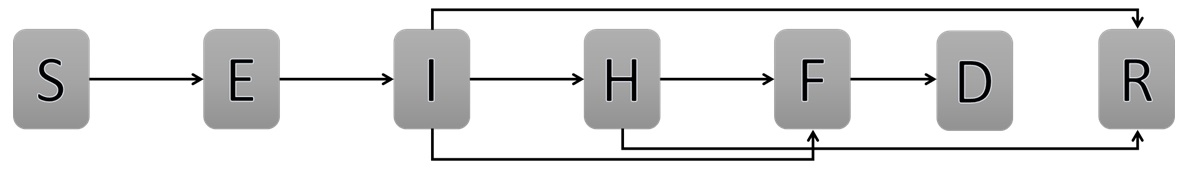
\includegraphics[width=1\textwidth]{compartmentNoFlow}
  \caption{Compartment Model of the Ebola Epidemic in Liberia \newline  Being S: Susceptible, E: Exposed, I: Infectious, H: Hospitalized, F: Funeral,  R: Recovered and D: Dead. } 
\label{fig:compartment} 
\end{figure}
\end{frame}

\begin{frame}
\frametitle{Assumptions}
\end{frame}

\begin{frame}
\frametitle{Parameters/Data}
\begin{figure}[!h]
  \centering
  %\includegraphics[width=1\textwidth]{tab_para}
  \caption{Model Parameters for Ebola Epidemic in Liberia Before and After the International Intervention. Calibrated parameters are written in bold font, and posterior means and standard deviations in parenthesis are notated. } 
\label{fig:compartment} 
\end{figure}
\end{frame}

\begin{frame}
\frametitle{Parameters/Data}
\begin{figure}[!h]
  \centering
  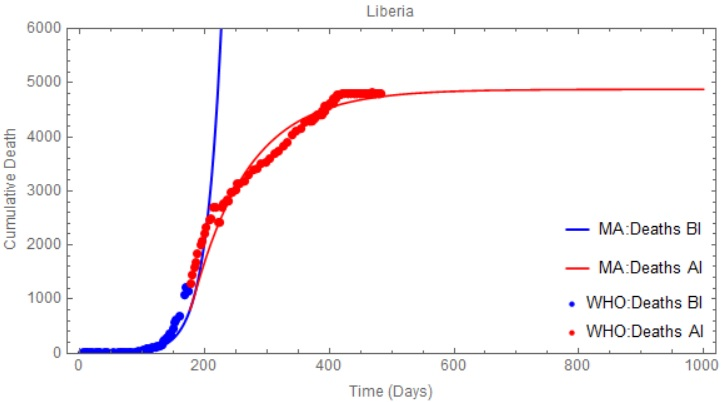
\includegraphics[width=1\textwidth]{CumulativeDeathMathematica}
  \caption{Validation of calibration. Dots represent cumulative death data and the lines represent simulation
based on mean posterior parameters. (Blue) - pre intervention and (red) - post treatment.} 
\end{figure}
\end{frame}


\begin{frame}
\frametitle{System model}
\section{System}
Should we add equations?
\end{frame}

\begin{frame}
\frametitle{System Model Results}
\begin{figure}[!h]
  \centering
  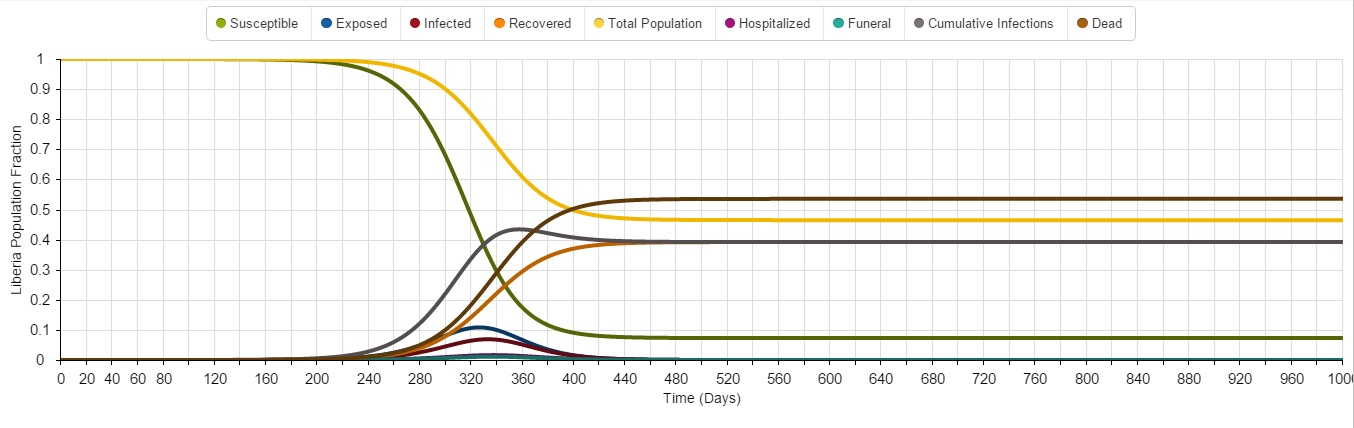
\includegraphics[width=1\textwidth]{LB_NoInt_SD_IM}
  \caption{ Insight Maker results using the parameters of the first stage (Mar/14 to Sept/14) and assuming no intervention}
\label{fig:LB_IM_NoIn} 
\end{figure}
\end{frame}

\begin{frame}
\frametitle{System Model Results}
\begin{figure}[!h]
  \centering
  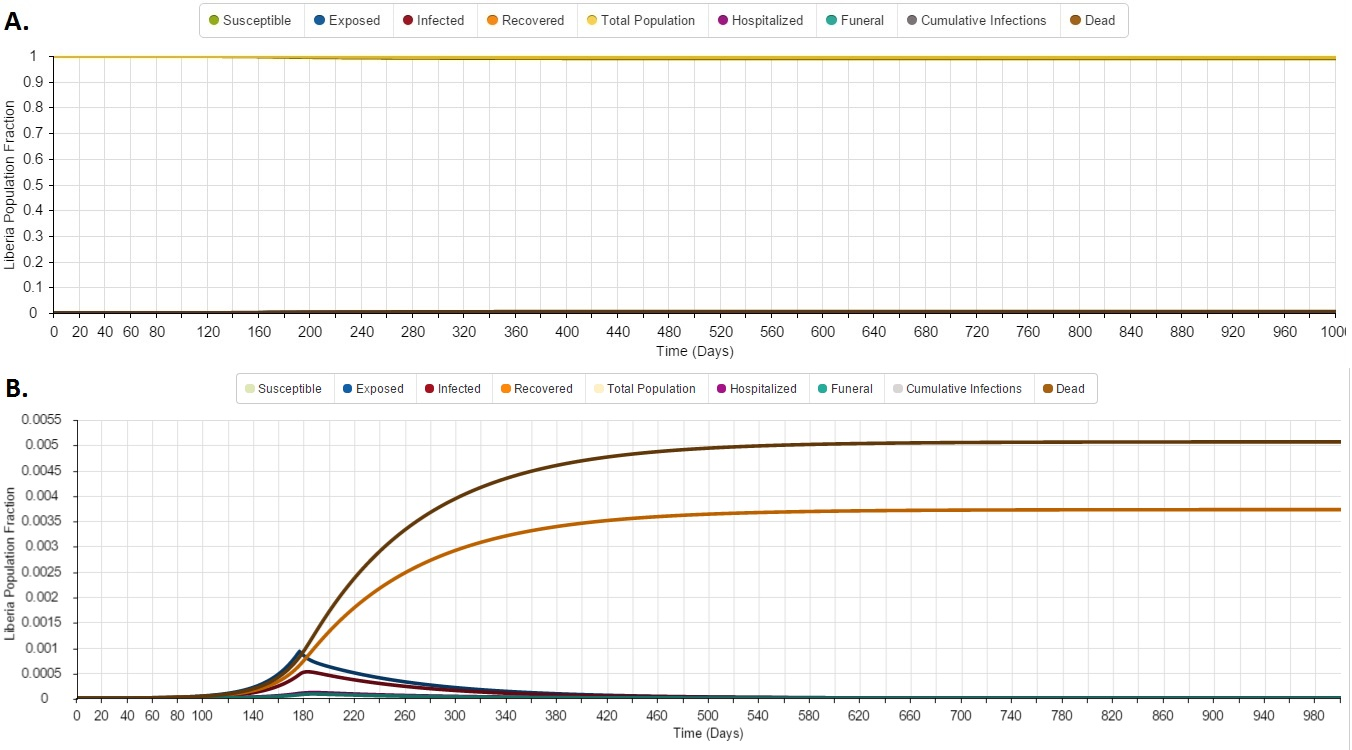
\includegraphics[width=1\textwidth]{LB_Int3_SD_IM}
  \caption{ Insight Maker results. \textit{Top:} parameters of the first stage (Mar/14 to Sept/14), \textit{Bottom:} parameters of the second stage ( Sept/14 to July/15)}
\label{fig:LB_IM_In} 
\end{figure}
\end{frame}

\begin{frame}
\frametitle{System Model Results}
\begin{figure}[!h]
  \centering
  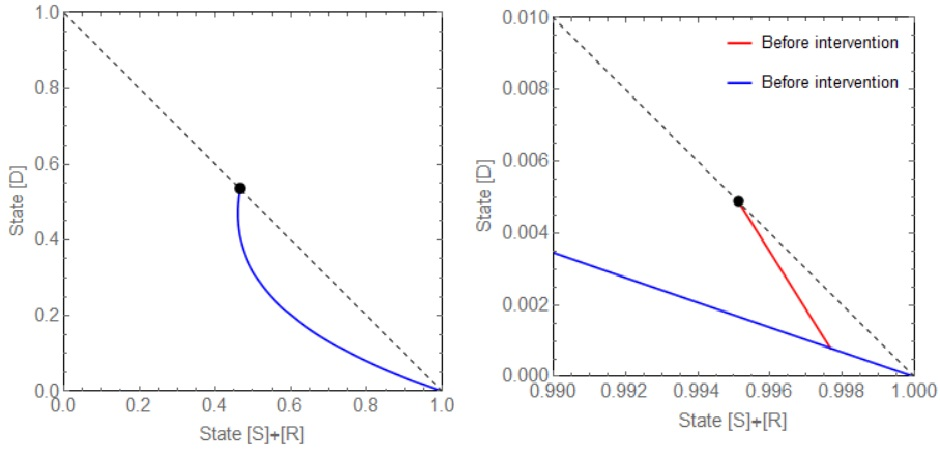
\includegraphics[width=1\textwidth]{PhasePortrait}
  \caption{ Projection of phase portrait to (Susceptible + Recovered, Dead) space. (Blue) - without intervention,
(Red) - with intervention, (Dots) - where the phase converges (equilibrium).}

\end{figure}
\end{frame}




\begin{frame}
\frametitle{Agent model}
\section{Agent}
%MAYBE INCLUDE DIAGRAM
%\begin{figure}
%\begin{tikzpicture}[->,>=stealth',shorten >=1pt,auto,node distance=3cm,
%  thick,main node/.style={circle,fill=blue!20,draw,font=\sffamily\Large\bfseries}]
%  \node[main node] (1) {S};
%  \node[main node] (2) [right of=1] {E};
%  \node[main node] (3) [right of=2] {I};
%  \node[main node] (4) [right of=3] {R};
%    \node[main node] (5) [below left of=3] {D};
%      \node[main node] (6) [below right of=3] {F};
%        \node[main node] (7) [right of=6] {H};
%
%  \path[every node/.style={font=\sffamily\small}]
%    (1)
%        edge node {$p_{SE}$} (2)
%        edge [loop above] node {$p_{SS}$} (1)
%    (2) 
%        edge node {$p_{EI}$} (3)
%         edge [loop above] node {$p_{EE}$} (2)
%      
%    (3) 
%       edge node {$p_{IR}$} (4)
%       edge node[left] {$p_{IF}$} (6)
%       edge node {$p_{IH}$} (7)
%        edge [loop above] node {$p_{II}$} (3)
%    (4)
%         edge [loop above] node {$p_{RR}$} (4)
%       
%(6) edge node{$p_{FD}$} (5) 
%edge [loop below] node {$p_{FF}$} (6)     
%(7) edge node[right]{$p_{HR}$} (4) 
%edge [loop below] node {$p_{HH}$} (7)
%  (7) edge node{$p_{HF}$} (6)      
% (5) edge [loop below] node {$p_{DD}$} (5)
%        ;
%\end{tikzpicture}
%\end{figure}
\begin{itemize}
\item \textbf{INCLUDE FLOW CHART ONE MORE TIME}
\item Probabilistic model vs. deterministic.
\item Flows become probabilities.
\item Individuals vs. system.
\begin{itemize}
\item 1000 individuals; 1 exsposed.
\item 500 days.
\item 100 repetitions.
\end{itemize}
\end{itemize}
\end{frame}


\begin{frame}
\frametitle{Agent Model Results}
30 percent of the time outbreak deoes not happen

\begin{figure}
  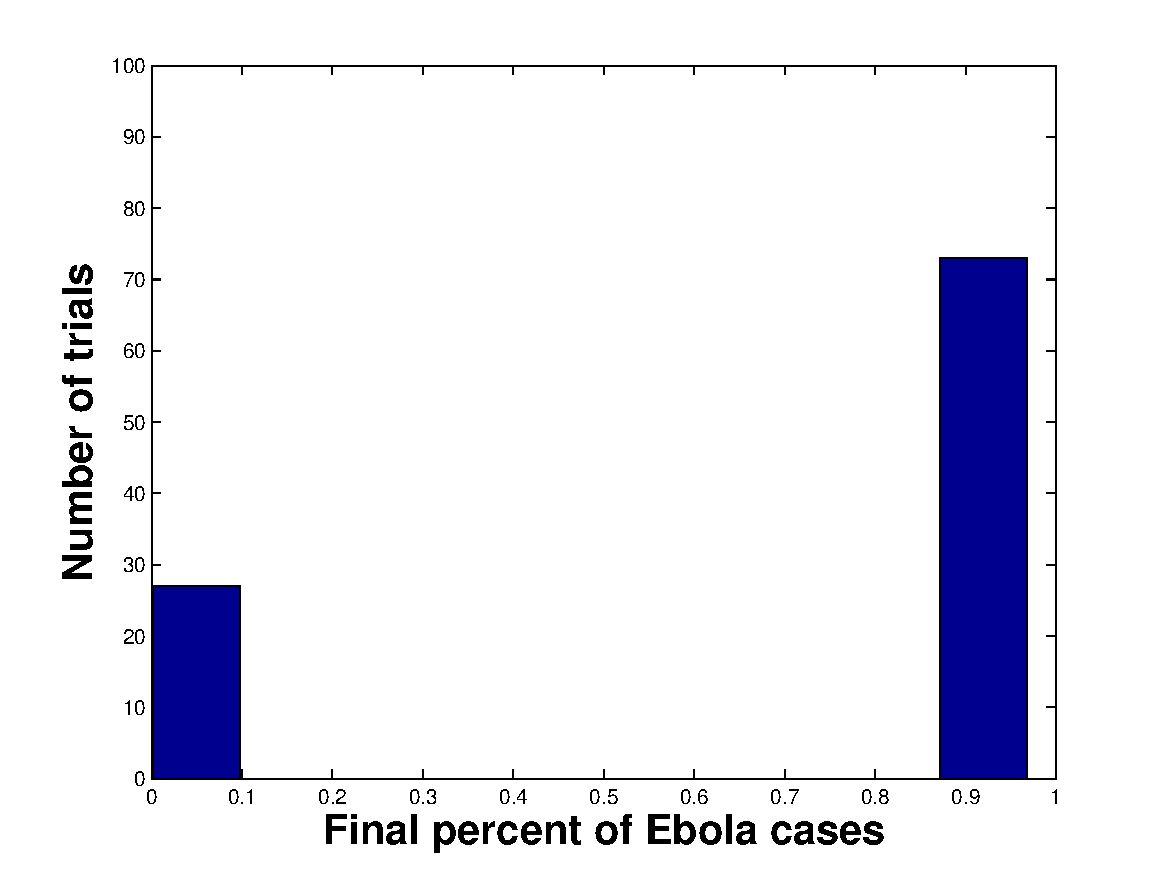
\includegraphics[scale=0.35]{N1000Hist-eps-converted-to} \caption{Progression of the proportion of the total population in Susceptible, Recovered and Dead states through time.}
% %
\end{figure}
\end{frame}


\begin{frame}
\frametitle{Agent Model Results}
\begin{itemize}
\item A typical outbreak will cause \textbf{HOW MANY} percent of the total population to get the disease.
\item Among those \textbf{HOW MANY DEAD}.
\end{itemize}

\begin{figure}
  %\includegraphics[scale=0.35]{TimeSeries} \caption{Progression of the proportion of the total population in Susceptible, Recovered and Dead states through time.}
% %
\end{figure}
\end{frame}


\begin{frame}
\frametitle{Agent Model Results}
%\textbf{PHASE PORTRAIT PICTURE}
\begin{figure}
  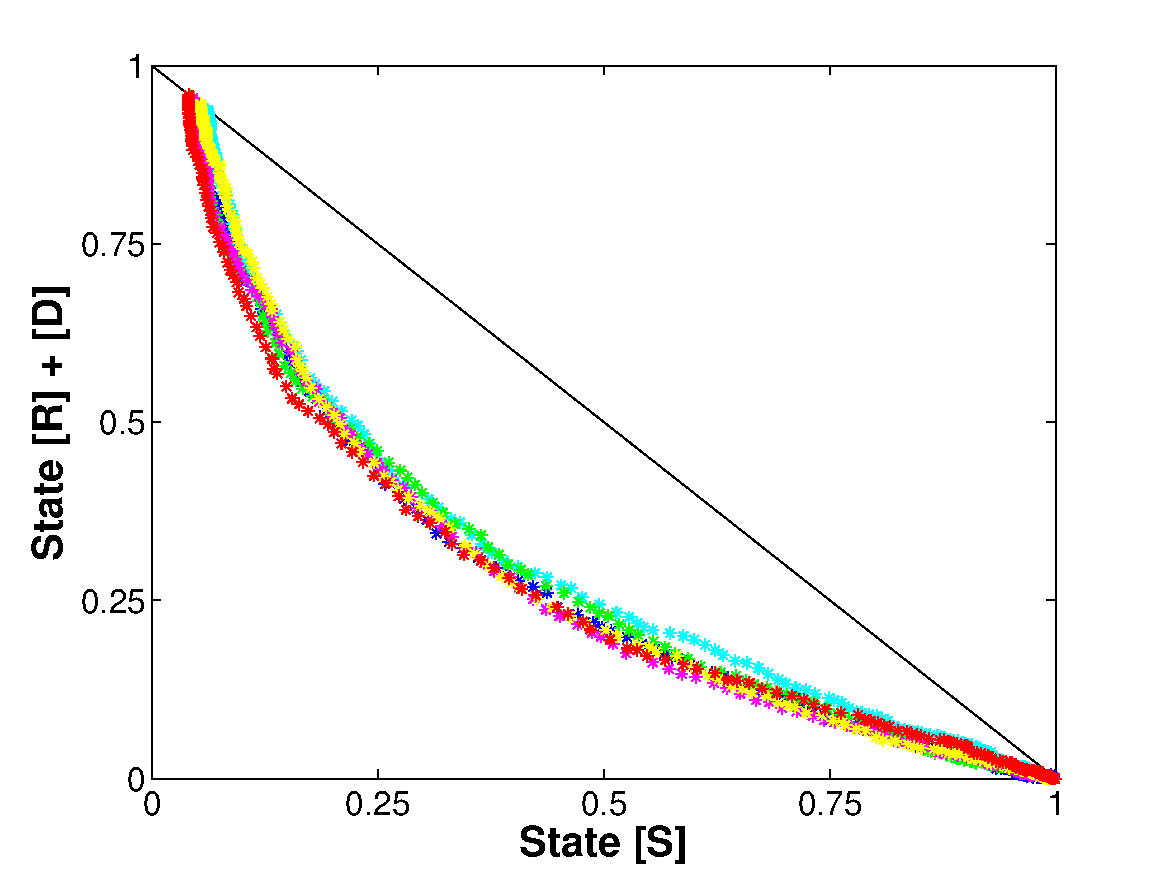
\includegraphics[scale=0.35]{PhasePortrait-eps-converted-to} \caption{Probabilistic Phase Portrait}
% %
\end{figure}
\end{frame}



\begin{frame}
\frametitle{Spatial Agent Model}
\section{Spatial}
\begin{itemize}
\item Why we should incorporate the spatial info?
\begin{itemize}
\item We have different contact ratios within households, communities and funerals ($\beta_H$, $\beta_C$, $\beta_F$)
\item Travel patterns are distinct among big cities and small villages
\end{itemize}
\item show the Flow Chart Models
\item go into the details of the model
\begin{itemize}
\item How people get infected (3 different scenarios: househoulds, communities and funerals)
\item How people travel (every one has prob 0.2 to travel, those away from home will return w/ prob 0.5, while the others have higher chance to travel locally, different probabilities based on the density of the cities/villages for non-local travellers)
\end{itemize}
\item Figures $\&$ results
\end{itemize}

\end{frame}

\begin{frame}{Spatial Importance}
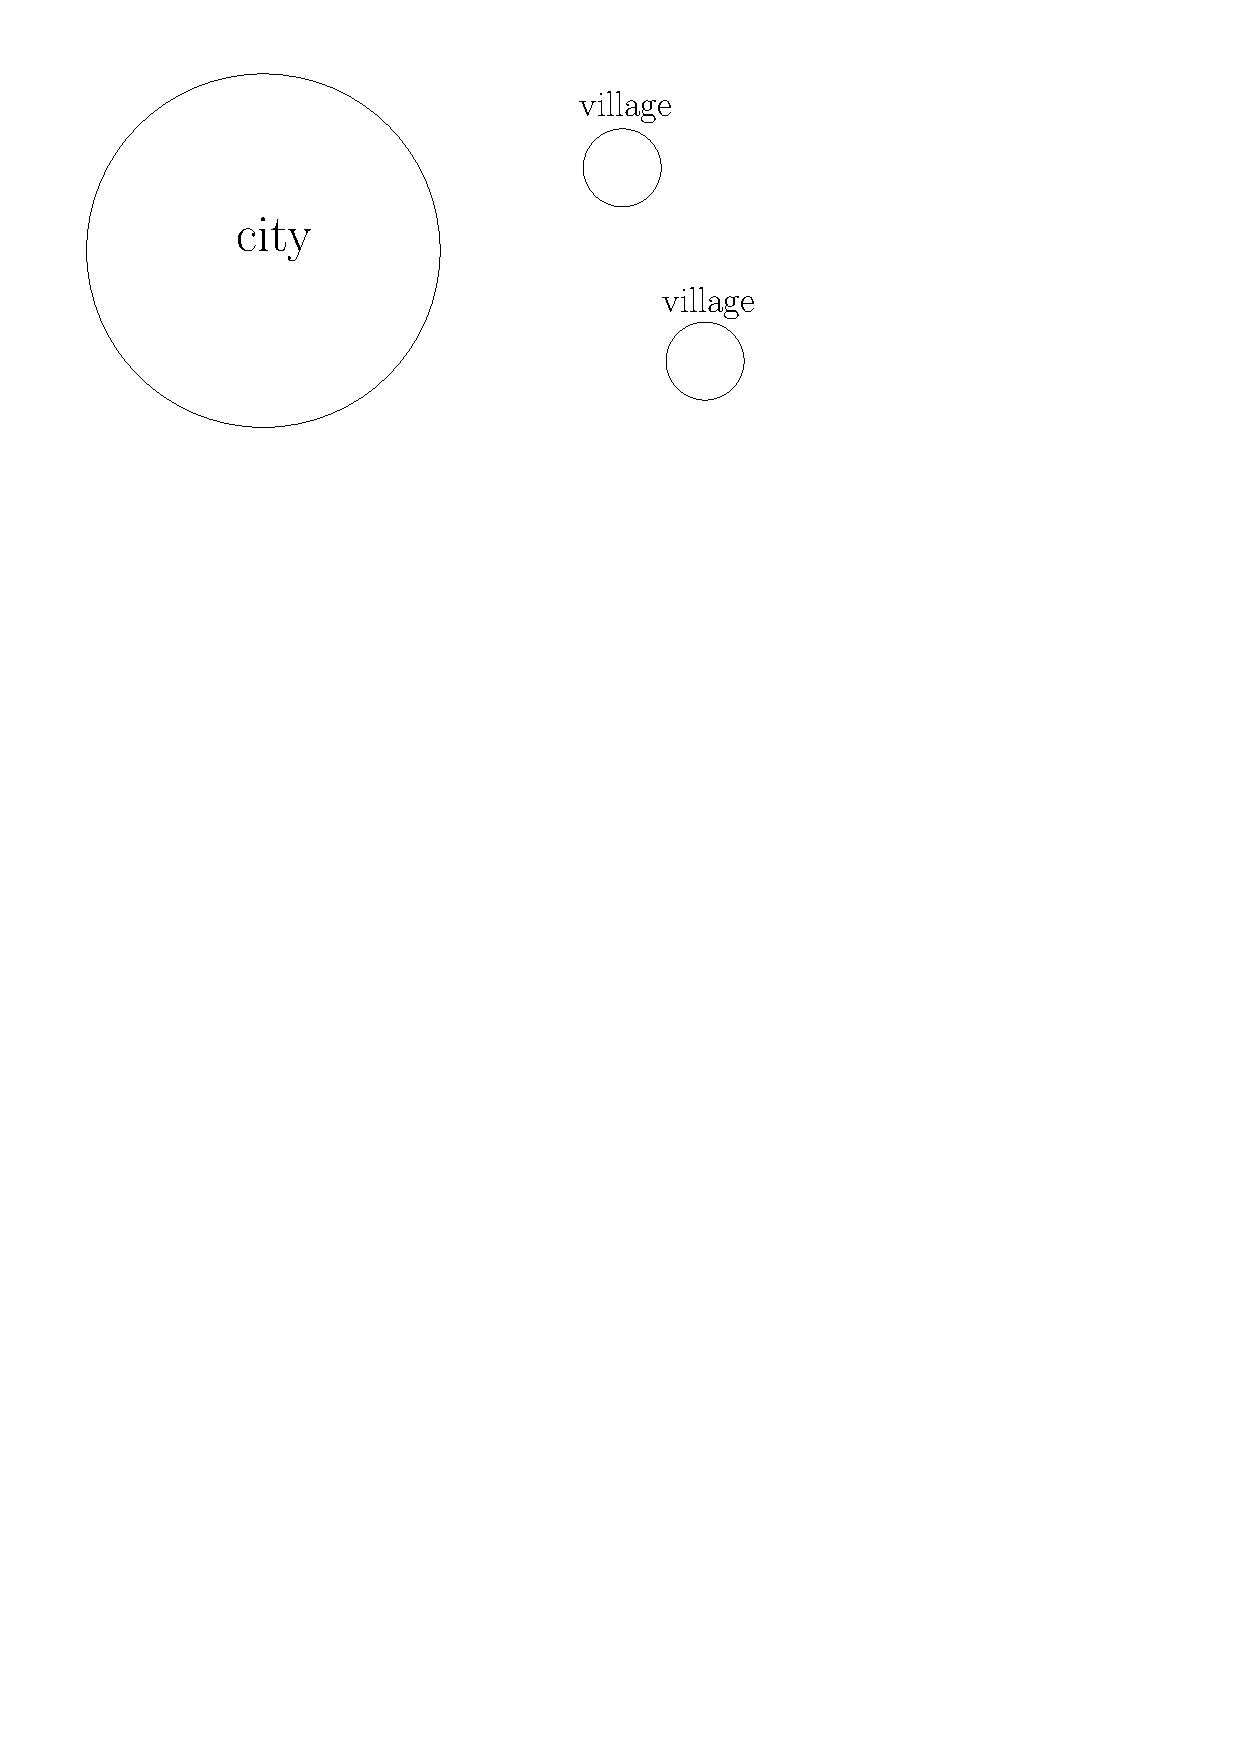
\includegraphics[width=\textwidth]{cities}
\end{frame}
%\draw[fill=black] (1,1) rectangle (2,2);

\begin{frame}{States and Transitions}
\begin{figure}[h!]
\begin{center}
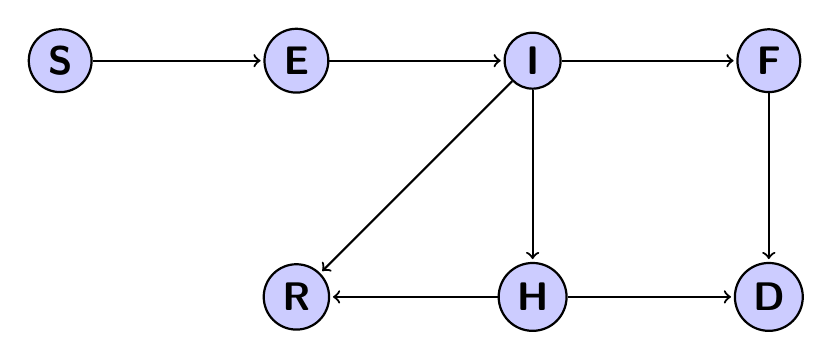
\begin{tikzpicture}[->,shorten >=1pt,auto,node distance=3cm,
  thick,main node/.style={circle,fill=blue!20,draw,font=\sffamily\Large\bfseries}]

  \node[main node] (1) {S};
  \node[main node] (2) [right of=1] {E};
  \node[main node] (3) [right of=2] {I};
  \node[main node] (4) [right of=3] {F};
  \node[main node] (5) [below of=3] {H};
  \node[main node] (6) [below of=4] {D};
  \node[main node] (7) [left of=5] {R};

  \path[every node/.style={font=\sffamily\small}]
    (1)
        edge node {} (2)
        %edge [loop above] node {$1-p_{SE}$} (1)
    (2) 
        edge node {} (3)
        % edge [loop above] node {} (2)
      
    (3) 
       edge node {} (4)
       edge node[right] {} (5)
       edge node[left] {} (7)
        %edge [loop above] node {$p_{II}$} (3)
    (4)
         edge node {} (6)
        % edge [loop above] node {$p_{FD}$} (6)
       
(5) edge node{} (6) 
	edge node {} (7)
%edge [loop below] node {$p_{FF}$} (6)     
;
        
\end{tikzpicture}
\end{center}
\caption{States and transitions for individuals.}
\label{fig:sabm-states}
\end{figure}
\end{frame}

\begin{frame}{Infection Rules}
%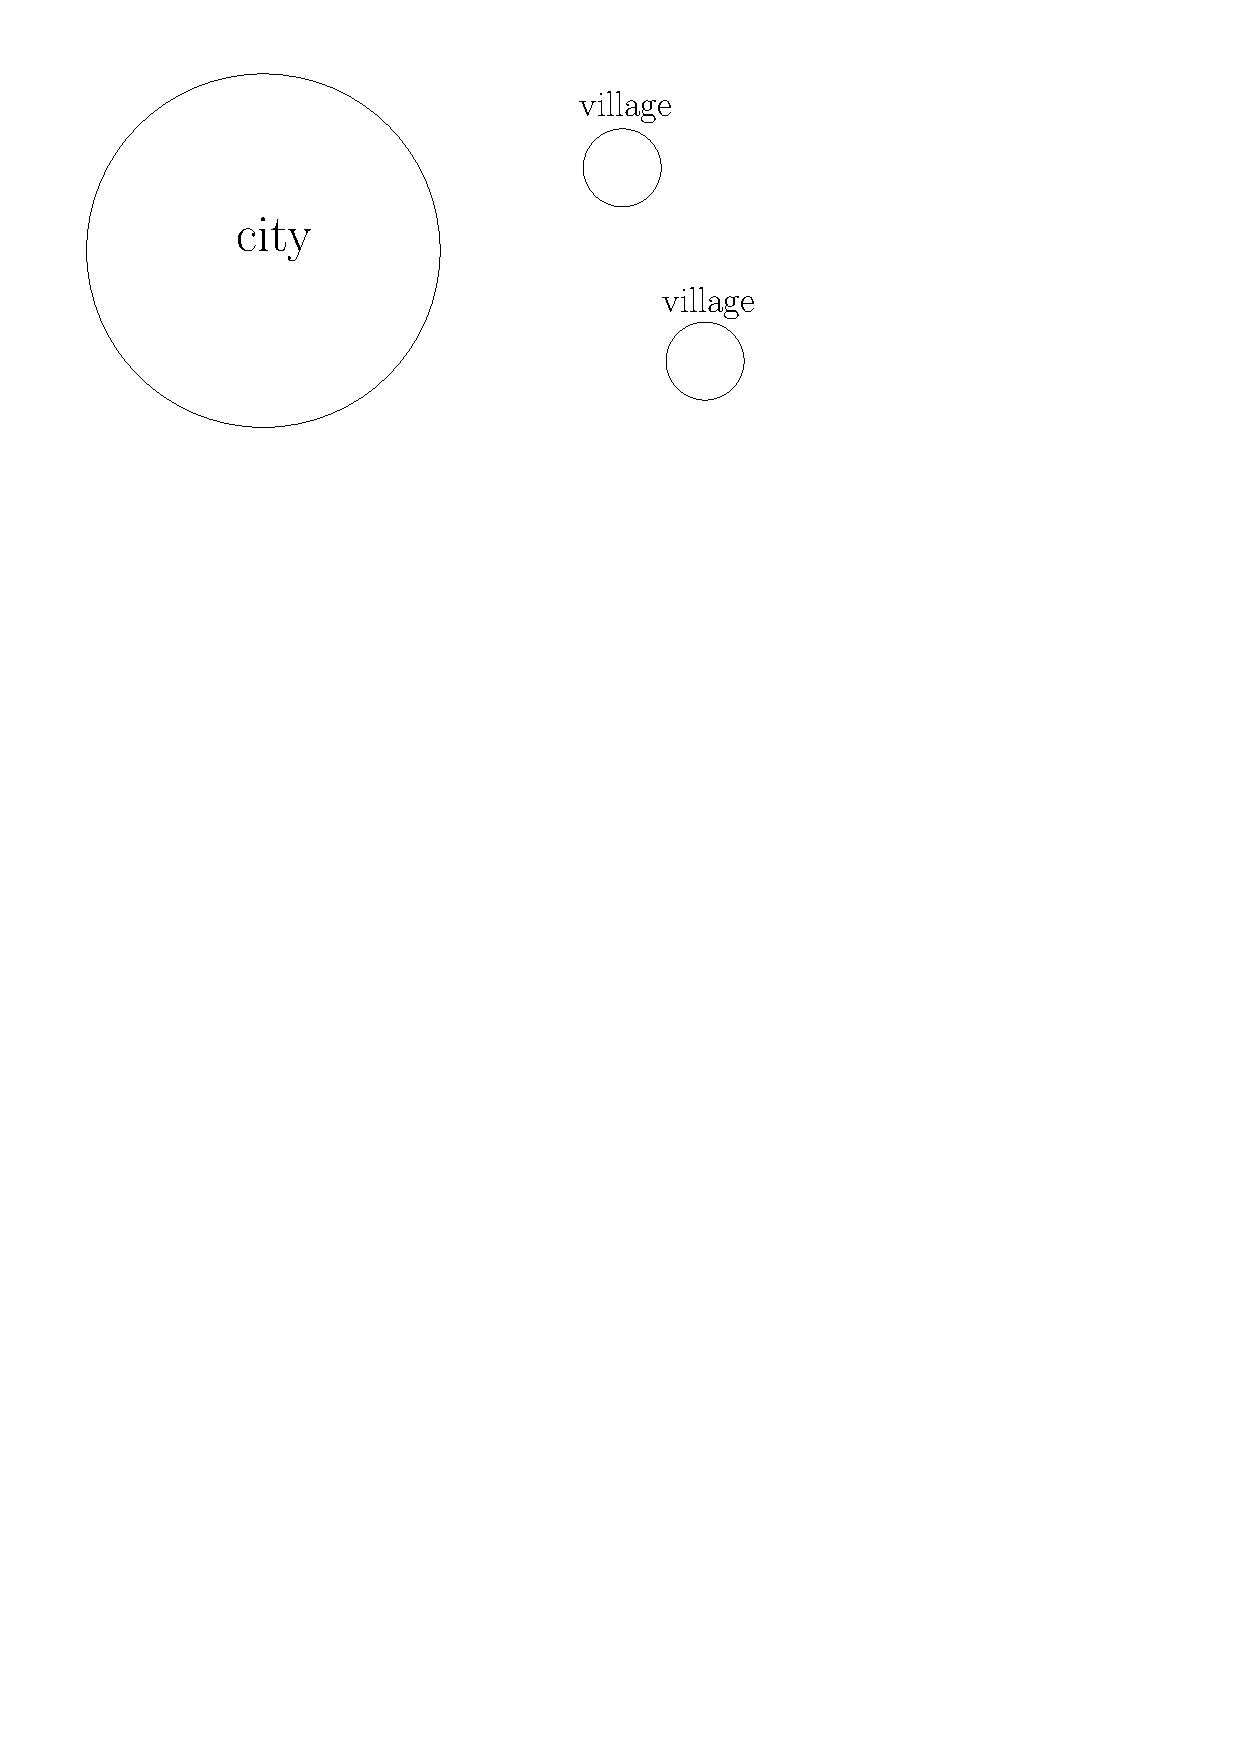
\includegraphics[width=\textwidth]{cities}
\begin{figure}[h!]
\begin{center}
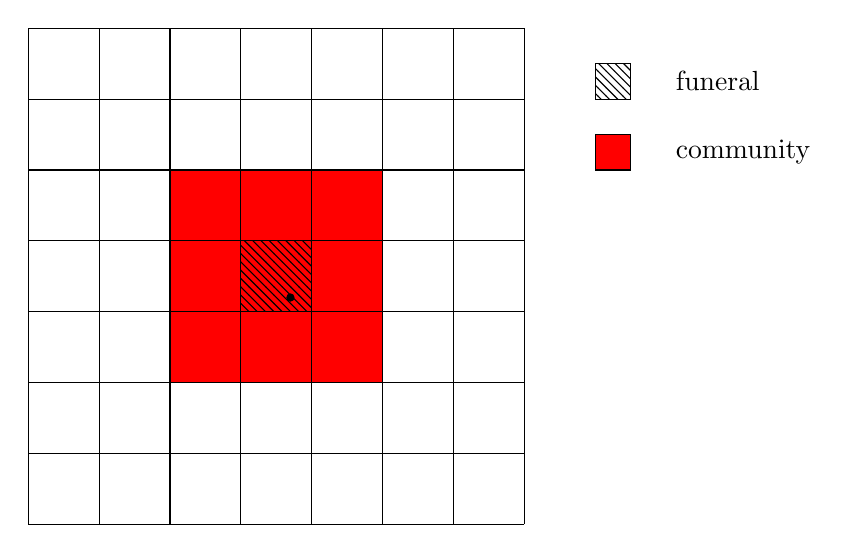
\begin{tikzpicture}[scale=.9]
\draw [fill=red] (0,0) rectangle (3,3);
\draw[pattern=north west lines, pattern color=black] (1,1) rectangle (2,2);
\draw[step=1cm, thin] (-2,-2) grid (5,5);
\draw[fill=black] (1.7,1.2) circle (.05cm);

\draw[pattern=north west lines, pattern color=black] (6,4) rectangle (6.5,4.5);
\node[anchor=west] at (7,4.25) {funeral};
\draw[fill=red] (6,3) rectangle (6.5,3.5);
\node[anchor=west] at (7,3.25) {community};
\end{tikzpicture}
\end{center}
\caption{States and transitions for individuals.}
\label{fig:sabm-states}
\end{figure}
\end{frame}

\begin{frame}{Travel Rules}
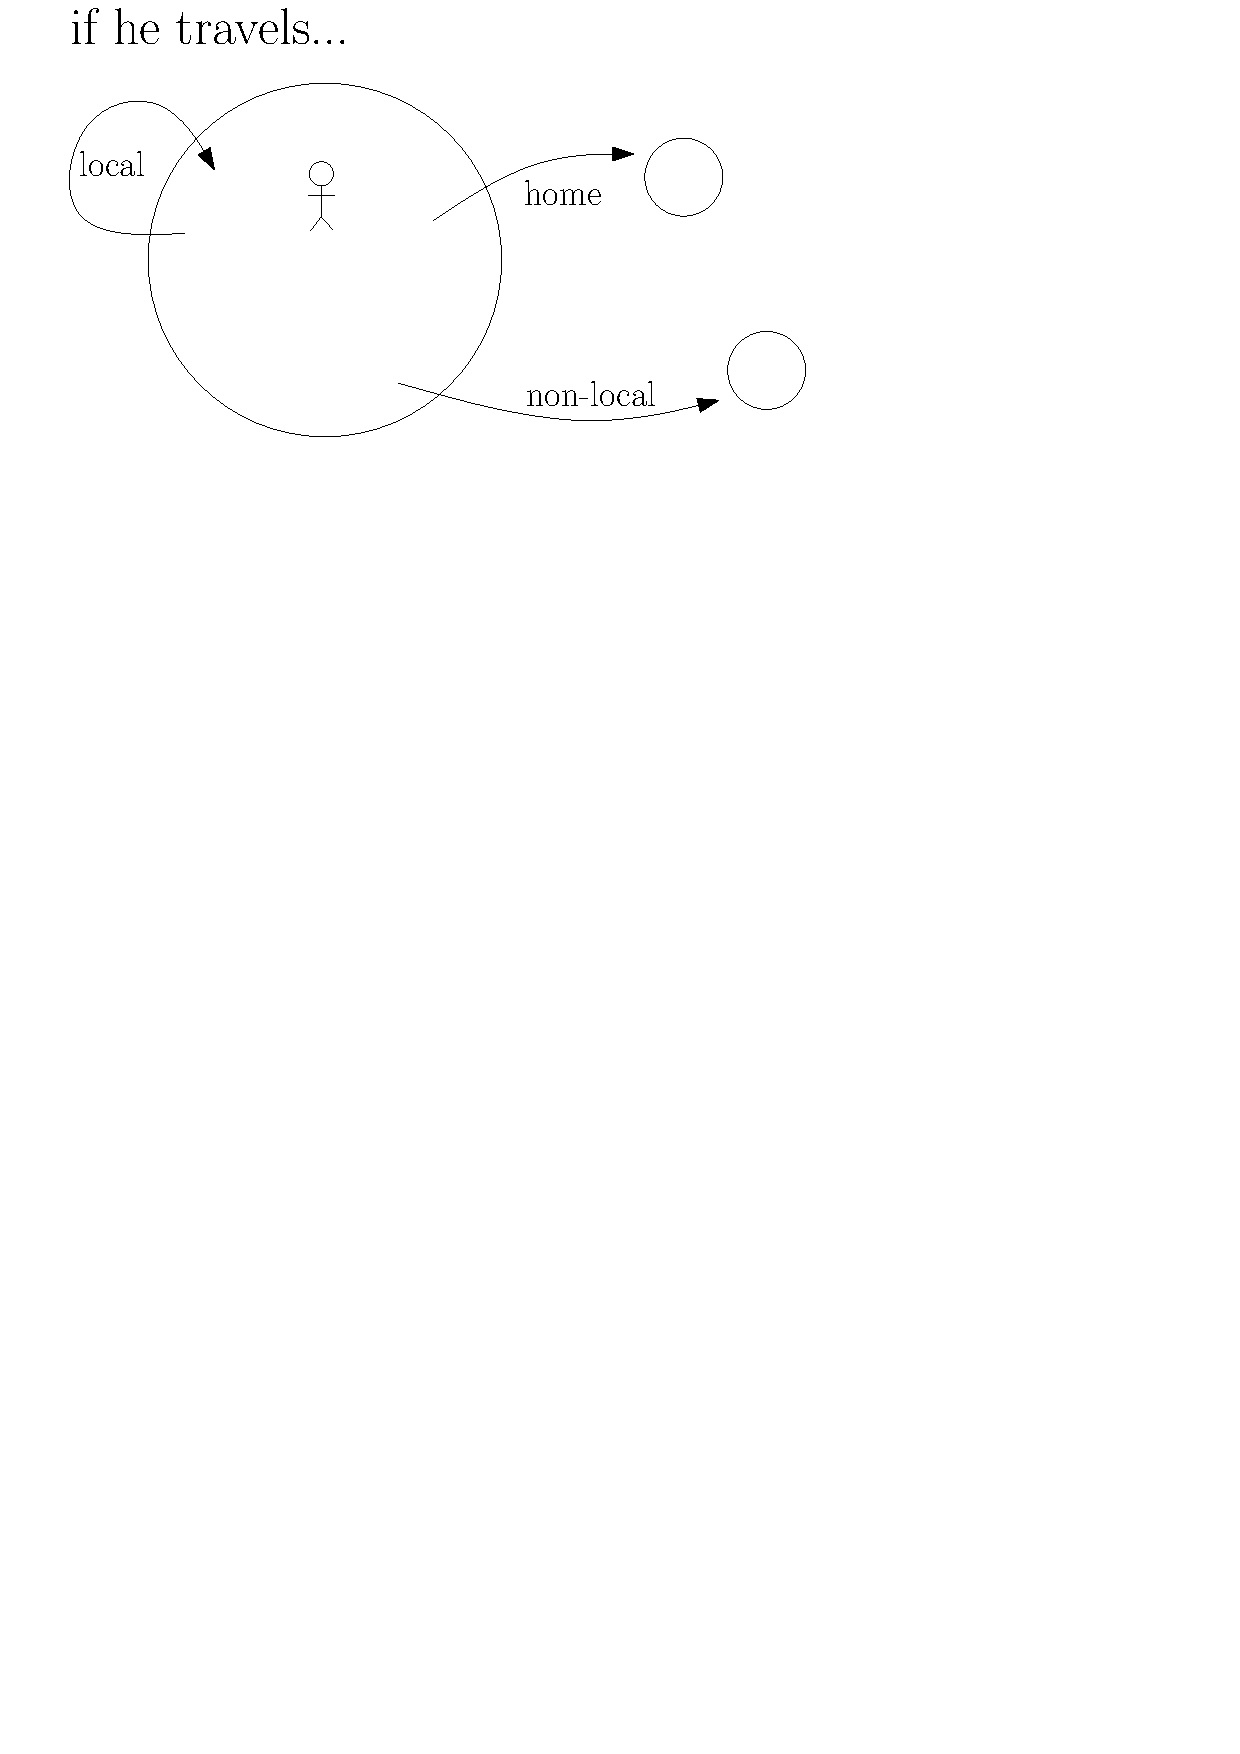
\includegraphics[width=\textwidth]{travel}
\end{frame}


\begin{frame}
\frametitle{Spatial Agent Model Results}
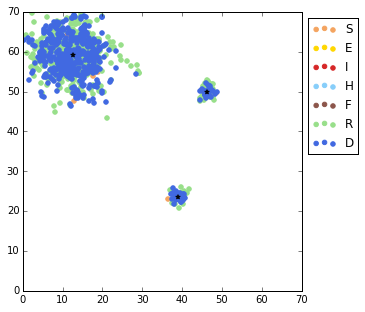
\includegraphics[width=.41\textwidth]{map1}
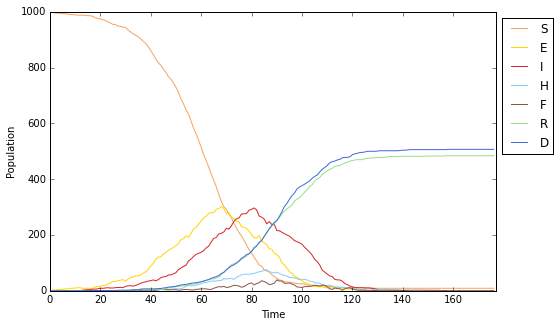
\includegraphics[width=.59\textwidth]{time1}
\end{frame}

\begin{frame}
\frametitle{Comparison}
\section{Comparison}
\end{frame}

\begin{frame}
\frametitle{Summary}
\section{Summary}
\end{frame}
\end{document}
